\section{Heating}
%\todo{Use \$ \$ for formulas and \textbackslash SI \{\}\{\} for the units}
\subsection{Requirements and Tasks}

% just an idea for now (Matthias)
To heat up the atoms to achieve a plasma and arrive at temperatures useful for experimentation, it is necessary to add a heating system to the reactor.
It was known already before that heating equipment using 2.45\,GHz microwave technology is probably the cheapest.
But it had to be elaborated if it can be fitted to the reactor, and what the price point is.
Also, it had to be verified, that the method is working for the parameters of the reactor to be built.
One more goal was to determine the parameters that could be achieved by means of the heating scheme.

\subsection{Outcome}
\subsubsection{Power balance}   % Matthias
To validate whether 2.45\,GHz heating will work, the density profiles had to be determined.
Those profiles, alongside the temperature profiles, were also of interest to get a glimpse of the parameters that the reactor will achieve upon successful implementation.

%0D omitted due to space constrains

% As a first step, a 0D simulation was performed according to \cite{plasmaParameterLimitsLechte2002}. 0D here means that the plasma parameters (temperature, density, diffusivities, heating power densities) were assumed to be constant over the plasma volume. Also, equilibrium was assumed, meaning that both input and output heat, as well as input and output particle numbers were assumed to be equal.

% For the intended design as outlined in the previous chapters, a plasma volume of $V = 0.04435\,\mathrm{m}^3$ was used. For the 0D-simulation, the heat diffusivity $\chi$ was assumed to be zero. This is fine, since it overall has a smaller impact on the simulations. The particle diffusivity $D$ was kept as a free parameter. The result is shown in  \autoref{fig:0d_volume04435_P1000} and \autoref{fig:0d_volume04435_P3000}.

% \begin{figure}
%   \center{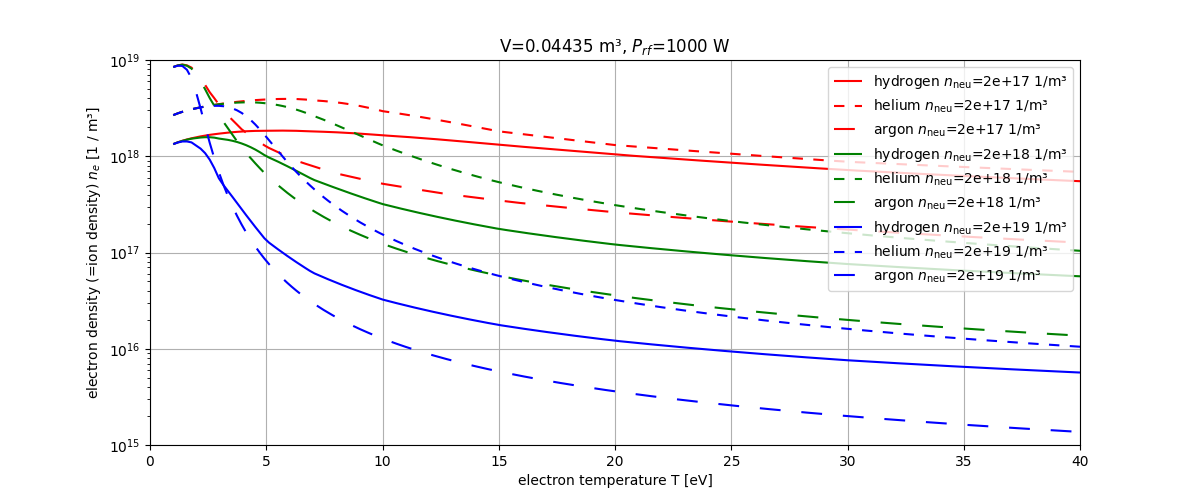
\includegraphics[width=12cm]{Images/05_Heating/0d_volume04435_P1000.png}}
%   \captionof{figure}{0D equilibrium varied over the particle diffusivity $D$, using a heating power of 1000\,W}
%   \label{fig:0d_volume04435_P1000}
% \end{figure}

% \begin{figure}
%   \center{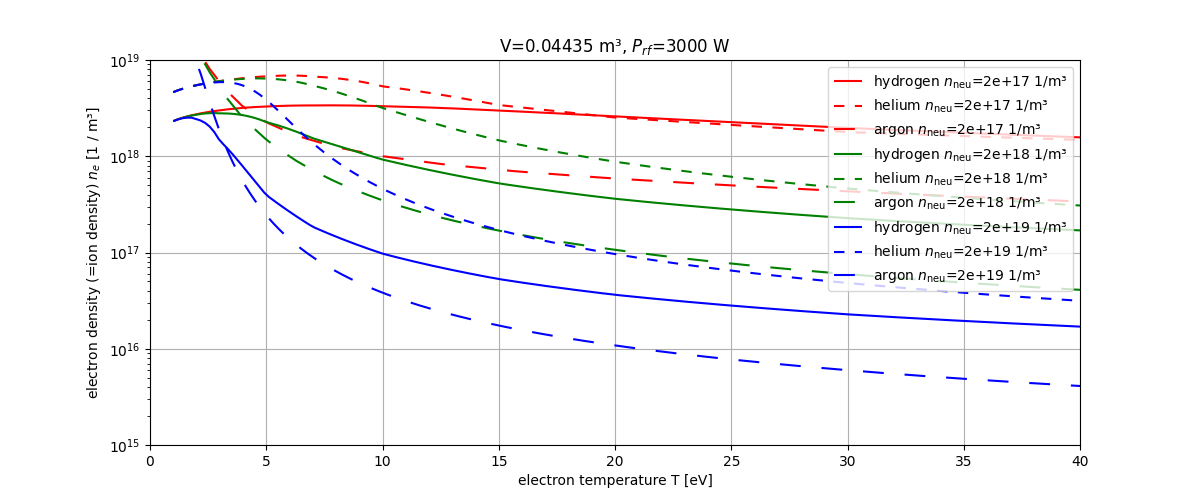
\includegraphics[width=12cm]{Images/05_Heating/0d_volume04435_P3000.png}}
%   \captionof{figure}{0D equilibrium varied over the particle diffusivity $D$, using heating power of 3000\,W}
%   \label{fig:0d_volume04435_P3000}
% \end{figure}

%It becomes clear that the lower the neutral density $n_\mathrm{neu}$, the lower the achievable electron densities. Another outcome is that the higher the heating power, the higher the input density.

\noindent From a preliminary 0D simulation implemented as described in \cite{plasmaParameterLimitsLechte2002}, it became clear that the lower the neutral density $n_\mathrm{neu}$, the lower the achievable electron densities.
Another outcome was that the higher the heating power, the higher the input density. \\

A 1D simulation, using the approach described in \cite{birkenmaierModeling2008}, was then performed.
Here, the major difference was, that the the plasma parameters were a function of the minor radius $r$.
Although the results presented here are at equilibrium, the 1D simulation also allows to calculate the profiles over time during the start phase. This is not used here since this would require to change the heating profile.

For the diffusivities and neutral densities, the parameters from the TJ-K experiment in Stuttgart were used, as shown in \autoref{tab:parameters}.

\begin{table}[H]
  \caption{1D simulation parameters. \\
  $D$ ... particle diffusivity \\
  $\chi$ ... heat diffusivity \\
  $n_new$ ... neutral density}
  \centering
  \begin{tabular}{lSS}
                                              & {Helium}               & {Argon}                 \\
    \hline
    $D$ / $\si{\meter\squared\per\second}$    & 8.5                   & 6                     \\
    $\chi$ / $\si{\meter\squared\per\second}$ & 200                   & 8                     \\
    $n_\mathrm{new}$                          & 2.30 $\times 10^{18}$ & 2.32 $\times 10^{17}$ \\
  \end{tabular}
  \label{tab:parameters}
\end{table}

%It should be noted that the TJ-K only achieved up to 10\,eV, while the 1D simulations presented here predict around 40\,eV for some configurations. Also, the fits for the cross sections stated in \cite{plasmaParameterLimitsLechte2002} are only valid for up to 40\,eV, which is slightly surpassed by some simulations.

\autoref{fig:1d_volume04435_argon} shows the resulting temperature and density profiles, assuming that all the heating power can be deposited into the plasma without losses. The profiles for Helium have the same shape, but the maximum temperature is 47\,eV instead of 32\,eV, and the maximum density is $0.58 \times 10^{18} \, \si{\meter^{-3}}$ instead of $1.23 \times 10^{18} \, \si{\meter^{-3}}$.

% \begin{figure}[H]
%   \center{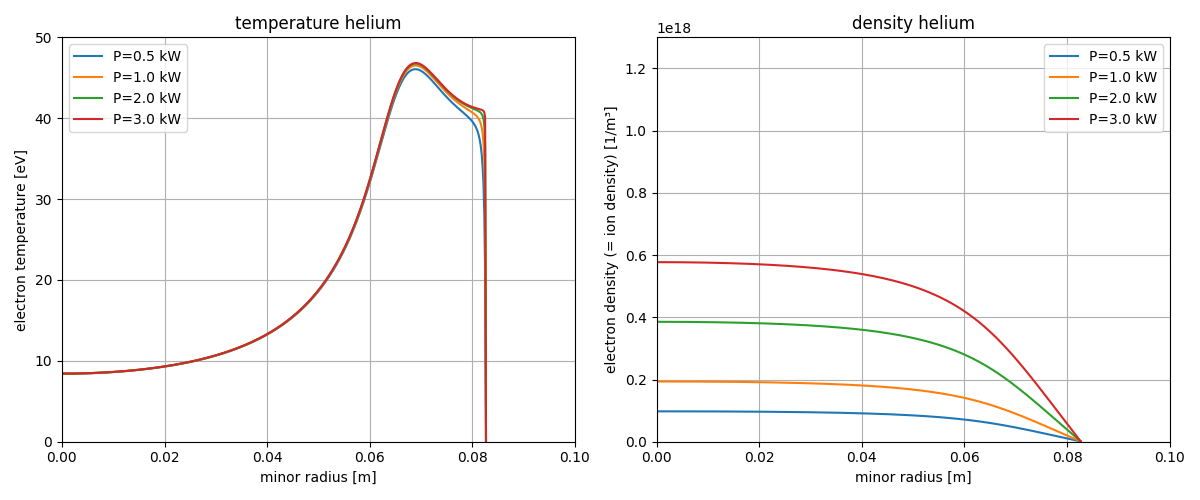
\includegraphics[width=12cm]{Images/05_Heating/1d_volume04435_helium.png}}
%   \captionof{figure}{1D equilibrium radial profiles for Helium.}
%   \label{fig:1d_volume04435_helium}
% \end{figure}

\begin{figure}[H]
  \center{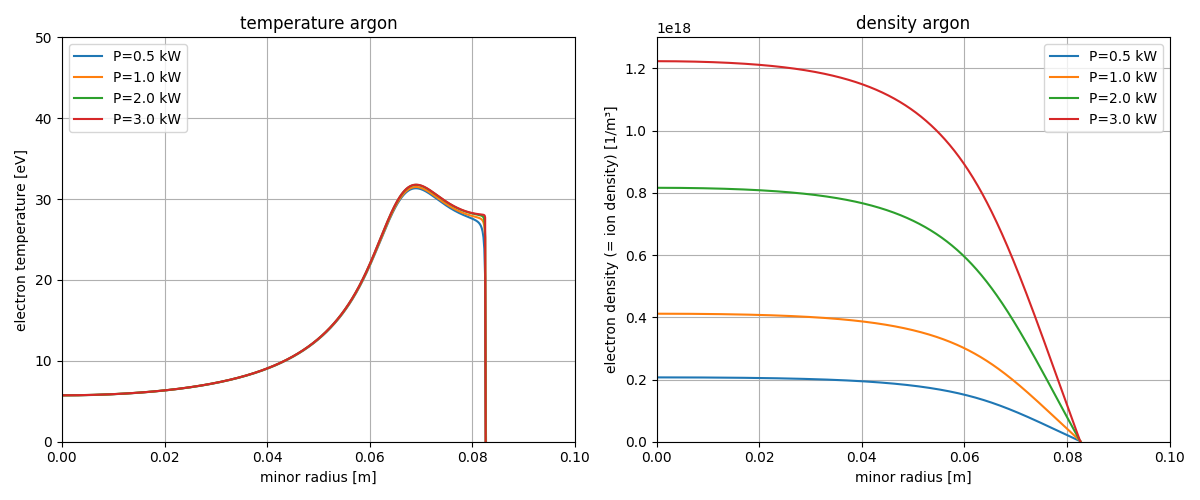
\includegraphics[width=14cm]{Images/05_Heating/1d_volume04435_argon.png}}
  \captionof{figure}{1D equilibrium radial profiles for Argon.}
  \label{fig:1d_volume04435_argon}
\end{figure}

\par One interesting outcome is that the temperature profile seems to be almost independent from the heating power.
This can be explained by the fact that at the heating profile, there is an equilibrium between newly ionized particles and ``lost'' particles due to diffusion (towards the plasma core and towards the plasma edge).
For this, one should take into account the average time $\tau$ that an ion spends in the heating zone before floating away due to diffusion.
As soon as the average power deposited per particle per dwell time $\tau$ reaches the ionization energy, ionization will dominate, taking away all the excess energy.
Only below 100\,W, the temperature begins to sink when reducing the heating power further.
% Only at the start, there is such a small amount of ionized particles, that there will be a very high amount of energy per ionized particle, that cannot taken away by ionization processes fast enough - therefore we then have temperaatures much higher than 45eV at the heating zone

\par Also, the gradient at the outer edge is probably steeper than it would be in the experiment. Here, the reason is likely that the diffusion profiles taken from \cite{birkenmaierModeling2008} are for temperatures around 10\,eV instead of 30\,eV, and therefore too low for the presented machine.

\subsubsection{Heating processes}  % Diogo
In order to recreate how the heating would occur, a series of theoretical approximations were made.
To start with, even though this is a design of a stellarator, a toroidal symmetry was assumed.
Then, the density profile was assumed to be parabolic and poloidally centred and the magnetic field to decay with $1/r$.
It was also assumed that the frequency of the wave sent into the plasma was much higher than the ion cyclotron (IC) frequency ($\omega >> \omega_{ci}$), so the dynamics of the ions, which are much slower than the electrons, was overall neglected. \\

The interest is to have an overdense plasma, $\omega_{pe} > \omega_{ce}$ everywhere, making it impossible to heat up the plasma only by exciting the electron cyclotron resonance (ECR).
This is because the incoming wave will be reflected at the critical density, where the wave reaches $\omega_{pe}$.
There will also have to be excitation of the upper-hybrid resonance (UHR), but, when plasmas are overdense, the R-wave that permits this heating method is also reflected back at the $\omega_R$ cut-off before reaching this mode.
These frequency profiles can be seen in \autoref{fig:freq_profiles}.
In the end, a combination of these heating processes, alongside with O-X-B heating will be necessary in order to heat up the plasma.
The O-X-B process consists of having an O-wave ($\overrightarrow{E_1} // \overrightarrow{B_0}$) propagate into the plasma until being reflected at $\omega_{pe}$ and converted into an X-wave ($\overrightarrow{E_1} \perp \overrightarrow{B_0}$).
In turn, this X-wave propagates in the direction contrary of emission until being reflected back again at $\omega_R$ and converted into a Bernstein wave.   
This wave can finally cross through the $\omega_{pe}$ cut-off frequency and reach the position in the plasma where ECR heating (ECRH) can occur.
In practice, however, we expect the heating radiation to disperse throughout the vacuum vessel, being reflected off of the walls (and having its polarity change) and absorbed through various other processes.

\begin{figure}[H]
  \centering
  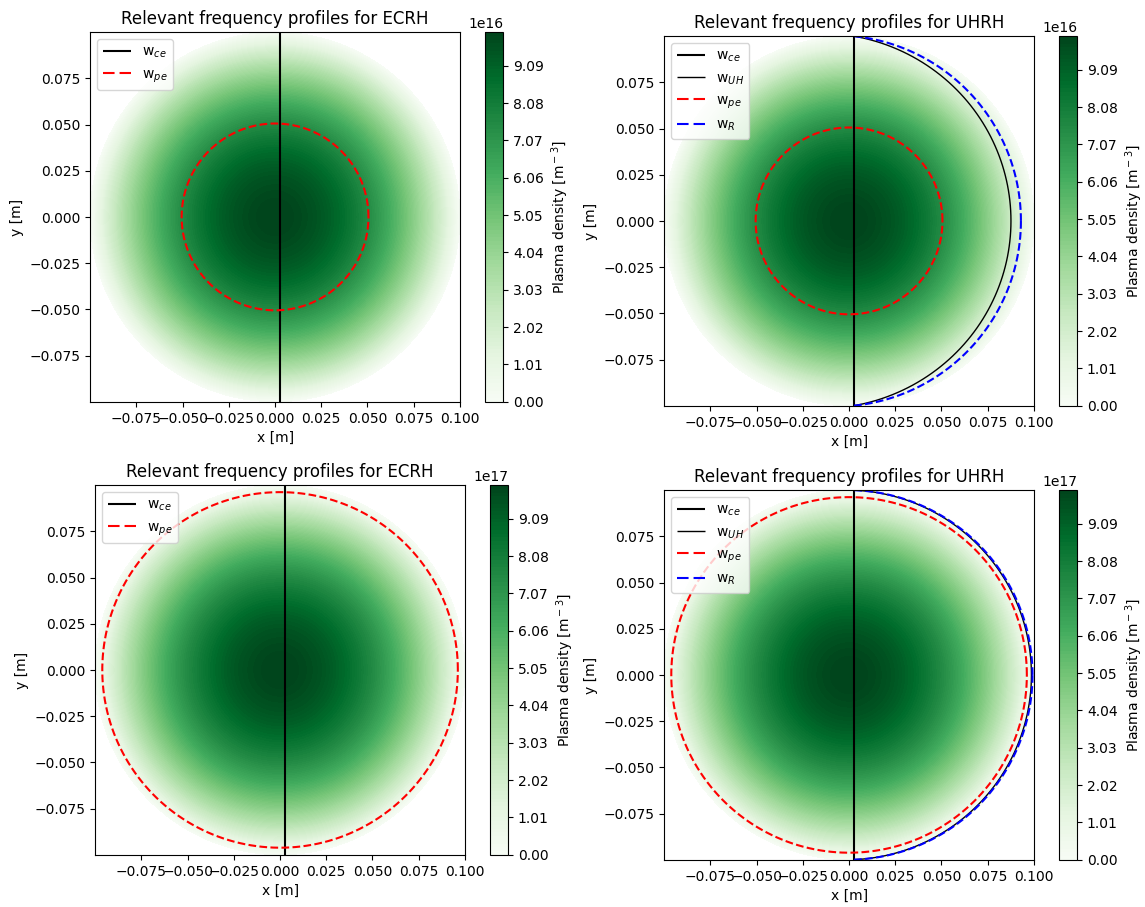
\includegraphics[width=0.8\textwidth]{Images/05_Heating/freq_profiles.png}
  \caption{Frequency profiles for ECRH and UHRH for non overdense (top) and overdense (bottom) plasma. The resonant frequencies $\omega_{ce}$ and $\omega_{UH}$ and the cut-off frequencies $\omega_{pe}$ and $\omega_R$ are displayed.}
  \label{fig:freq_profiles}
\end{figure}




\subsubsection{Hardware}    % Joe

The 2.45\,GHz microwaves will be generated by a magnetron, and transported to the plasma by WR340 waveguides (86.36 x 43.18)\,mm. This size was chosen to maintain polarization by only allowing the TE1 mode to propagate. Upon reaching the vacuum chamber, the microwaves will be focused using an optimum horn antenna. It is important for effective heating, that the wider H-plane flare is oriented along the vertical axis perpendicular to the containment B-field.
Further RF components must be added along the waveguides to minimize feedback into the magnetron. A circulator and a directional coupler are added to remove any returning waves. A 3-stub tuner is added before the horn antenna to maximize the heating system's efficiency.
\subsection{Outlook}
In the end, further developments can still be made.
In regard to the cross-sectional wave resonance and cut off profiles, only the example of a tokamak was studied.
This was enough to understand what will qualitatively happen, upon heating of the plasma, but the quantitative study is not applicable to a stellarator design.
Further work on this could then consist of figuring out which cross section of the stellarator is most ideal to perform heating on, depending on its shape.

% Still missing: Joe & Matthias


\subsection{Learnings}

% Matthias
One of the main learnings from the simulations were that the major two parameters to achieve are higher densities are heating power, but also the neutral density $n_\mathrm{new}$.
A more technical learning was, that while \cite{birkenmaierModeling2008} employed the Crank-Nicelson scheme for numerical implementation, a naïve fully-explicit scheme works as well.
The only downside was, that around 500 times more steps were needed.
But the python/numpy-based implementation still took less than 5 minutes per case (depending on number of radial points).
